
\clearpage
\section{Benutzerverwaltung}

\begin{wrapfigure}[6]{l}{6.5cm}   % [x] Wie manche Zeile soll sich um die Grafik "brechen"
  \vspace{-35pt}      % Grundwert war 20; mit 30 schön oben beim Text ausgerichtet
  \begin{center}
    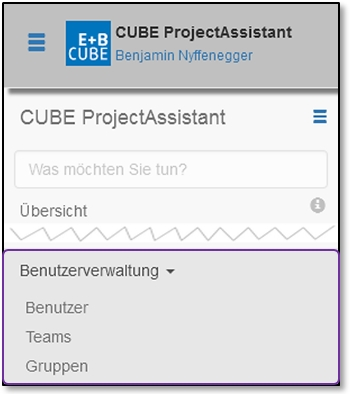
\includegraphics[width=1\linewidth]{../chapters/14_Benutzerverwaltung/pictures/14_Menu_Benutzerverwaltung.jpg}
  \end{center}
  \vspace{-20pt}
  \caption{Die Benutzerverwaltung verwenden}
  \vspace{-10pt}
\end{wrapfigure}

Wählen Sie im Menü links den Punkt 'Benutzerverwaltung'. Es erscheinen die Unterpunkte 'Benutzer', 'Teams' und 'Gruppen'.

\vspace{\baselineskip}

Die Benutzerverwaltung ist nur bei Personen eingeblendet, welche dafür berechtigt wurden. Sie wird ausschliesslich durch Administratoren verwaltet.

\vspace{4cm}  

\textbf{Übersicht:}

\vspace{.3cm}  

\textbf{Benutzer}: Bei den Benutzern werden sämtliche Personen, welche mit CUBE PA einen Berührungspunkt haben, erfasst. Hier erfolgen die Zuordnungen \ zu Tags, Sitzungsarten, Teams etc. Zudem wird festgelegt, ob ein Benutzer auch einen Zugang zum CUBE PA erhält oder nur bei Auswahlfeldern (bei Sitzungen, Beschaffungen, Dokumentenberechtigungen etc.) aufgelistet werden soll. Erfasste Benutzer können bei der Adressliste ausgeblendet werden. Ein wesentliches 'Steuerungselement' sind die Berechtigungsrollen, welche hier einem Benutzer gegeben werden können (z.B. Administrator).

\vspace{\baselineskip}

\textbf{Teams}: Es können Teams definiert werden, welchen Benutzer zugewiesen werden können (Einstellungen bei Benutzer).

\vspace{\baselineskip}

\textbf{Gruppen}: Hier werden Gruppen erstellt. In den Einstellungen der Gruppen können Benutzer, Teams und auch Beteiligte hinzugefügt werden. Zudem können einer Gruppe bestimmte Zugriffsrechte (Lesezugriff, Schreibzugriff, Löschzugriff) zugeordnet werden.

% \clearpage
\subsection{Benutzer}
\label{bkm:Ref445362390}

In der Übersicht der Benutzer kann wie gewohnt nach Begriffen gefiltert oder gesucht werden. Aufgelistete Benutzer können in der Benutzerverwaltung angezeigt oder bearbeitet werden. 

\vspace{\baselineskip}

In der Liste ist ersichtlich, wann sich ein Benutzer das letzte Mal im CUBE PA angemeldet hat. 

\begin{figure}[H]
\center{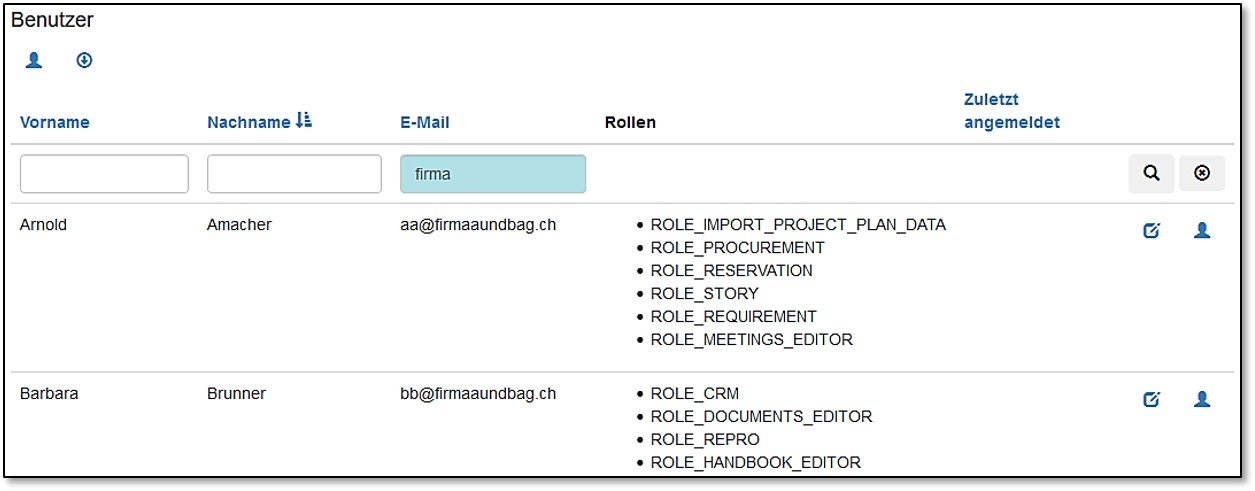
\includegraphics[width=1\linewidth]{../chapters/14_Benutzerverwaltung/pictures/14-1_Benutzeruebersicht.jpg}}
\caption{Übersicht der Benutzeradministration}
% \label{fig:speciation}
\end{figure}

Die Benutzerverwaltung sowie die Adressliste greifen auf dieselben Daten in der Datenbank zu. Grundsätzlich liegt bei der Benutzerverwaltung der Fokus auf den Benutzern, welche sich in CUBE PA einloggen können. Wie an entsprechender Stelle bei der Adressliste vermerkt, wird beim Erstellen einer Person in der Adressliste der Datensatz so angelegt, dass sich diese Person in CUBE PA \textbf{nicht} anmelden kann. 

\vspace{\baselineskip}

\textbf{Neuer Benutzer anlegen:} Soll ein neuer CUBE-Benutzer angelegt werden, wird zuerst (in der Benutzerübersicht) mit Klick auf 
\includegraphics[height=12pt]{/Icons/Person.jpg} eine neue Person angelegt. Nach dem Speichern (Erstellen) kann der Benutzer mit Klick auf 
\includegraphics[height=12pt]{/Icons/User.jpg} bearbeitet werden. Für die Anmeldung an CUBE braucht es eine gültige Email-Adresse und die Box 'Aktiviert' muss angewählt werden \col{(2)}. Der zukünftige CUBE Benutzer erhält nun eine Email.\\
Fügen Sie dem Benutzer die gewünschten Rollen, sowie die Gruppenzugehörigkeit hinzu.

\begin{figure}[H]
\center{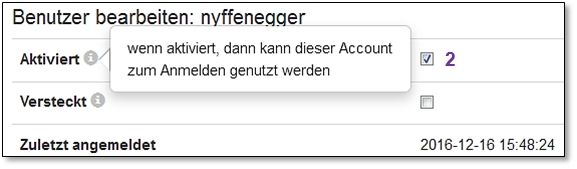
\includegraphics[width=.6\linewidth]{../chapters/14_Benutzerverwaltung/pictures/14-1_BenutzerAktivieren.jpg}}
\caption{Benutzeraccount aktivieren}
% \label{fig:speciation}
\end{figure}

Klicken Sie auf das Informations-Icon 
\includegraphics[height=12pt]{/Icons/Info_Hinweis.jpg}, um weitere Informationen zu den Einstellungen zu erhalten.

\vspace{-10pt}

% \clearpage
\subsubsection{Rollen}
\label{bkm:Ref445361985}

Folgende Rollen können einem Benutzer zugewiesen werden:

\begin{tabular}{|p{7.5cm}|p{7.5cm}|} % {c | p{14cm} l} %{cl}
\hline
\textbf{Rolle} & \textbf{Typ} \\
\hline	
ROLE\_IMPORT & ROLE\_USER \\
\hline
ROLE\_IMPORT\_PROJECT\_PLAN\_DATA & ROLE\_IMPORT \\
\hline
ROLE\_IMPORT\_TRANSACTION\_DATA & ROLE\_IMPORT \\
\hline
ROLE\_PROCUREMENT & ROLE\_USER \\
\hline
ROLE\_PROCUREMENT\_EXTENDED & ROLE\_PROCUREMENT \\
\hline
ROLE\_TRANSACTIONS & ROLE\_USER \\
\hline
ROLE\_TRANSACTIONS\_EDITOR & ROLE\_TRANSACTIONS \\
\hline
ROLE\_MEETINGS & ROLE\_USER \\
\hline
ROLE\_MEETINGS\_EDITOR & ROLE\_MEETINGS \\
\hline
ROLE\_HUMANRESOURCES & ROLE\_USER \\
\hline
ROLE\_HUMANRESOURCES\_EDITOR & ROLE\_HUMANRESOURCES \\
\hline
ROLE\_DOCUMENTS & ROLE\_USER \\
\hline
ROLE\_DOCUMENTS\_EDITOR & ROLE\_DOCUMENTS \\
\hline
ROLE\_ADDRESSLIST\_EDITOR & ROLE\_USER \\
\hline
ROLE\_HANDBOOK\_EDITOR & ROLE\_USER \\
\hline
ROLE\_SUPER\_USER & ROLE\_HUMANRESOURCES\_EDITOR, ROLE\_MEETINGS\_EDITOR, \newline ROLE\_TRANSACTIONS\_EDITOR, \newline ROLE\_PROCUREMENT\_EXTENDED, \newline ROLE\_DOCUMENTS\_EDITOR, \newline ROLE\_ADDRESSLIST\_EDITOR, \newline ROLE\_HANDBOOK\_EDITOR \\
\hline
ROLE\_ADMIN & ROLE\_USER, \newline ROLE\_ADDRESSLIST\_EDITOR \\
\hline
ROLE\_SUPER\_ADMIN & ROLE\_ADMIN, \newline ROLE\_IMPORT\_PROJECT\_PLAN\_DATA, ROLE\_IMPORT\_TRANSACTION\_DATA, ROLE\_PROCUREMENT\_EXTENDED,
\newline ROLE\_MEETINGS, \newline ROLE\_MEETINGS\_EDITOR, \newline ROLE\_TRANSACTIONS\_EDITOR, \newline ROLE\_HUMANRESOURCES\_EDITOR,
\newline ROLE\_DOCUMENTS\_EDITOR, \newline ROLE\_ADDRESSLIST\_EDITOR, \newline ROLE\_HANDBOOK\_EDITOR \\
\hline
ROLE\_UPGRADE & ROLE\_USER \\
\hline
\end{tabular}

\begin{itemize}
\item
Der Rolle-Typ~'ROLE\_USER' ist die unterste Ebene der Berechtigungen und wird einem Benutzer beim erstmaligen Anmelden automatisch zugewiesen.
\item
ROLE\_A: ROLE\_B: Diese Rollenvergabe bedeutet, dass der Benutzer mit Rolle A auch über die Rolle B verfügt.
\item
ROLE\_X: [ROLE\_Y, ROLE\_Z]: Diese Rollenvergabe bedeutet, dass der Benutzer mit Rolle X ebenso über die Rollen in den Klammern verfügt (Y und Z).
\end{itemize}

\subsubsection{Übersicht über 'Benutzer bearbeiten'}

\vspace{\baselineskip}
\vspace{\baselineskip}

\begin{wrapfigure}[7]{r}{9cm}
\vspace{-55pt}
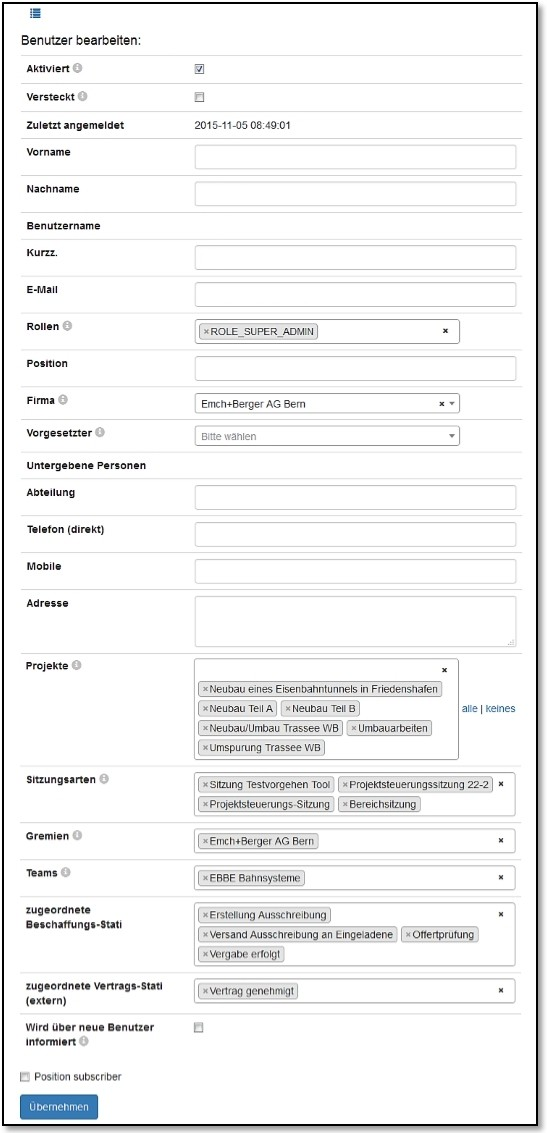
\includegraphics[height=185mm]{../chapters/14_Benutzerverwaltung/pictures/14-1-1_BenutzerBearbeiten.jpg}
% \caption{Status ändern}
\end{wrapfigure}

\begin{small}
\begin{raggedright}

Der angelegte Benutzer kann sich an CUBE PA anmelden

\vspace{\baselineskip}

\mbox{Benutzer soll in der Adressliste,} 
\mbox{sowie bei den Auswahlfenstern}
nicht erscheinen

\vspace{\baselineskip}

Zuweisen der verschiedenen CUBE PA \
Rollen (siehe Kapitel \ref{bkm:Ref445361985})

\vspace{\baselineskip}
\vspace{\baselineskip}
\vspace{\baselineskip}

Dem Benutzer können

\vspace{\baselineskip}

\begin{itemize}
\item Tags
\vspace{\baselineskip}
\vspace{\baselineskip}
\item Sitzungstypen
\vspace{\baselineskip}
\item Komitees
\item Teams
\item und Prozessschritte
\item und Statis beim \newline Beschaffungswesen
\end{itemize}

\vspace{\baselineskip}

zugewiesen werden.

\end{raggedright}
\end{small}

\raggedright{}

\clearpage
\textbf{Funktionshinweise}

\begin{figure}[H]
\center{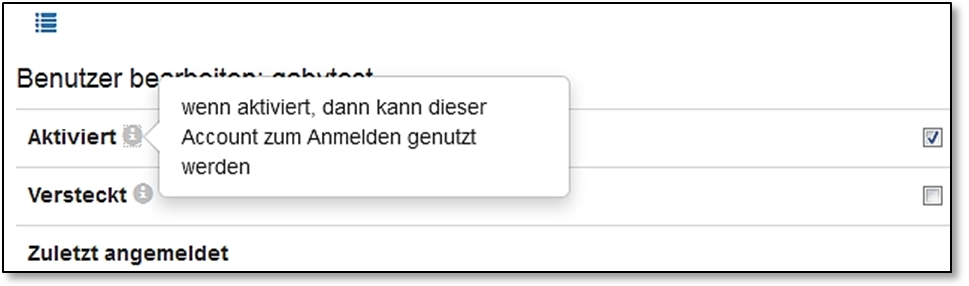
\includegraphics[width=0.6\linewidth]{../chapters/14_Benutzerverwaltung/pictures/14-1-1_Funktionshinweise.jpg}}
\caption{Funktionshinweise}
% \label{fig:speciation}
\end{figure}

Bei verschiedenen Feldern finden Sie ein 'i'-Symbol 
\includegraphics[height=12pt]{/Icons/Info_Hinweis.jpg}. Mit Klick auf dieses Symbol erhalten Sie Funktionshinweise über das entsprechende Eingabefeld.

\subsubsection{Beschaffungs- und Vertragsüberwachung konfigurieren}
\label{bkm:Ref20190318001}

In der persönlichen Projektübersicht können benutzerspezifisch Beschaffungs- und Vertragsüberwachungen angezeigt werden. Sobald eine Beschaffung oder ein Vertrag ein bestimmter Status, welcher einem Benutzer zugewiesen wurde, erreicht, wird ihm die Beschaffung, respektive der Vertrag auf der persönlichen Projektübersicht angezeigt.

\vspace{\baselineskip}

Für die Vertragsüberwachung müssen in der Datenbank bei 'Vertragsstatus (extern)' Status eingerichtet werden (die Funktionalität setzt auch ein Status-Workflow für die Beschaffungen voraus). In der 'Benutzerverwaltung' - 'Benutzer' werden die erforderlichen Status zugewiesen:

\begin{figure}[H]
\center{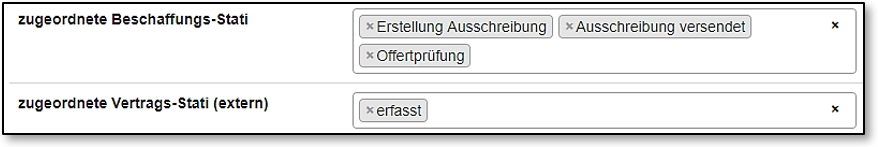
\includegraphics[width=0.8\linewidth]{../chapters/14_Benutzerverwaltung/pictures/benkonf_Besch-Vertr-Status.jpg}}
\caption{Beschaffungs- und Vertragsüberwachung einrichten}
% \label{fig:speciation}
\end{figure}

Beim Vertrageintrag ist ein 'Überwacher' oder/und 'Stv. Überwacher' zu definieren \col{(1)}:

\begin{figure}[H]
\center{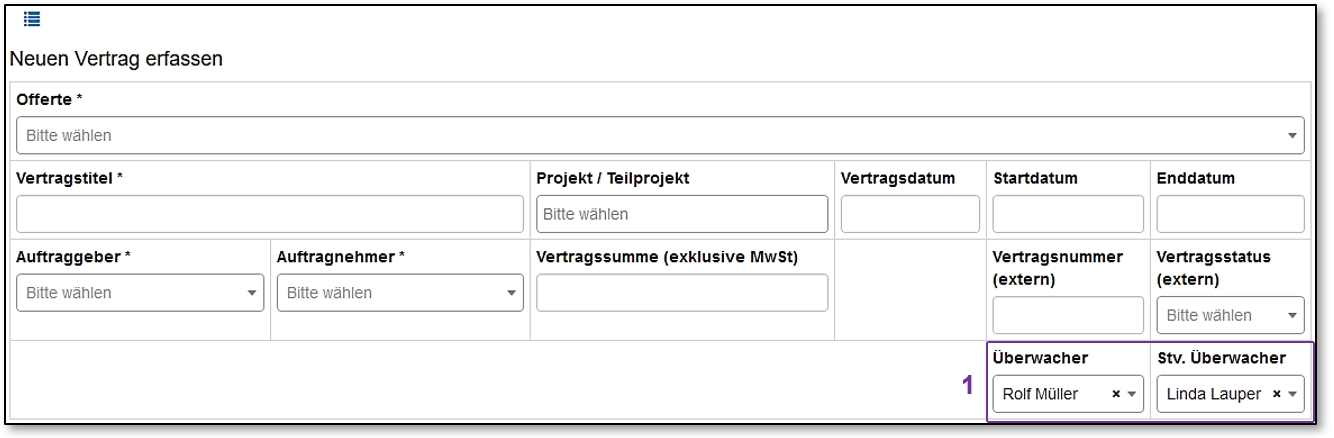
\includegraphics[width=1\linewidth]{../chapters/14_Benutzerverwaltung/pictures/benkonf_Vertrag.jpg}}
\caption{Beschaffungs- und Vertragsüberwachung einrichten}
% \label{fig:speciation}
\end{figure}



\pagebreak
\subsection{Teams}

Die Teams, welche hier erstellt werden können den Benutzern (siehe Kapitel \ref{bkm:Ref445362390}) zugewiesen werden.

\begin{figure}[H]
\center{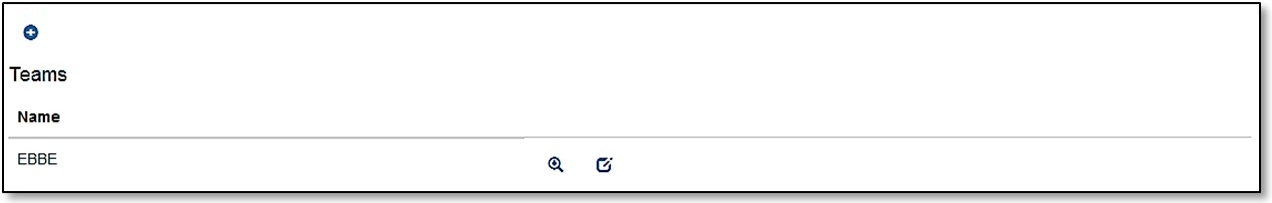
\includegraphics[width=1\linewidth]{../chapters/14_Benutzerverwaltung/pictures/14-2_TeamsUebersicht.jpg}}
\caption{Übersicht der erstellten Teams}
% \label{fig:speciation}
\end{figure}

\begin{figure}[H]
\center{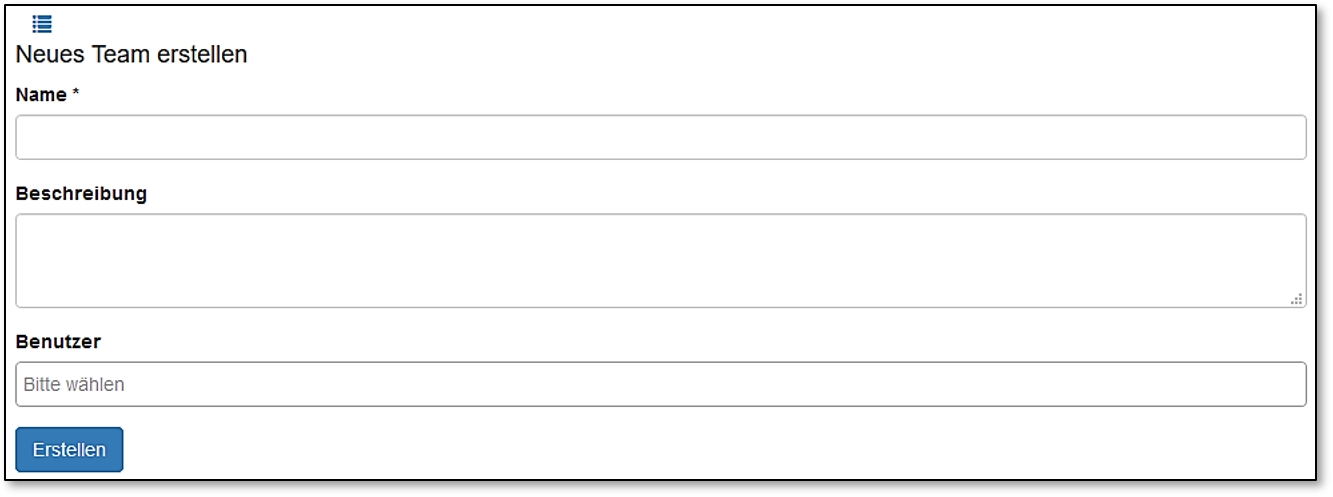
\includegraphics[width=1\linewidth]{../chapters/14_Benutzerverwaltung/pictures/14-2_TeamsBearbeiten.jpg}}
\caption{Bearbeitungsmodus der Teams}
% \label{fig:speciation}
\end{figure}

\clearpage
\subsection{Gruppen}

Hier werden Gruppen erstellt. In den Einstellungen der Gruppen können Benutzer, Teams und auch Beteiligte hinzugefügt werden. Zudem können einer Gruppe bestimmte Zugriffsrechte (Lesezugriff, Schreibzugriff, Löschzugriff) zugeordnet werden.

\begin{figure}[H]
\center{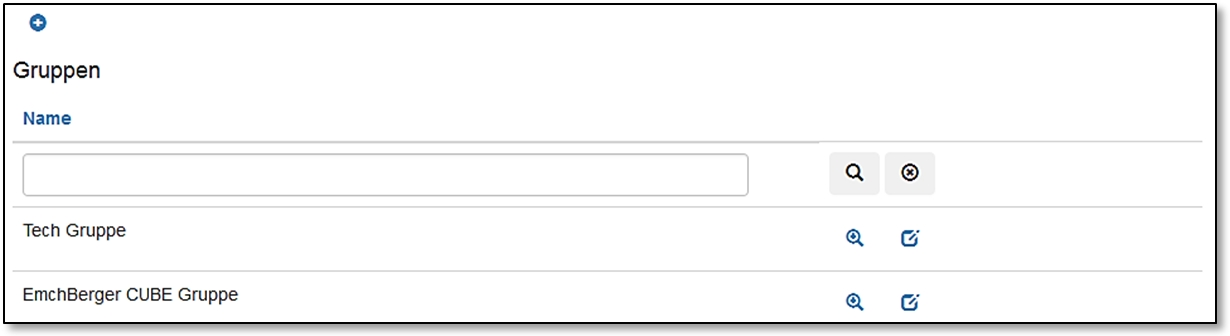
\includegraphics[width=1\linewidth]{../chapters/14_Benutzerverwaltung/pictures/14-3_GruppenUebersicht.jpg}}
\caption{Liste Gruppe}
% \label{fig:speciation}
\end{figure}

\begin{figure}[H]
\center{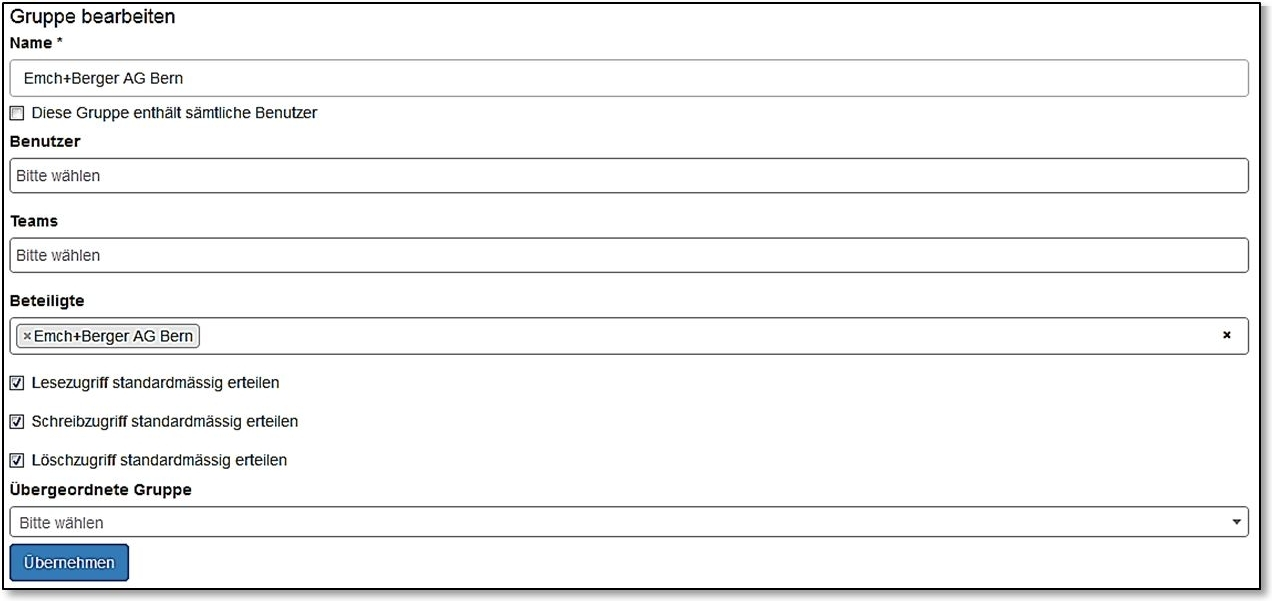
\includegraphics[width=1\linewidth]{../chapters/14_Benutzerverwaltung/pictures/14-3_GruppenBearbeiten.jpg}}
\caption{Bearbeitungsmodus der Gruppen}
% \label{fig:speciation}
\end{figure}

Gruppen können nebst einzelnen Benutzern auch Gruppen enthalten (Übergeordnete Gruppe). In der Dokumentenablage können bei den Gruppen-Berechtigungen explizit Untergruppen berechtigt oder ausgeschlossen werden \col{(1)}:

\begin{figure}[H]
\center{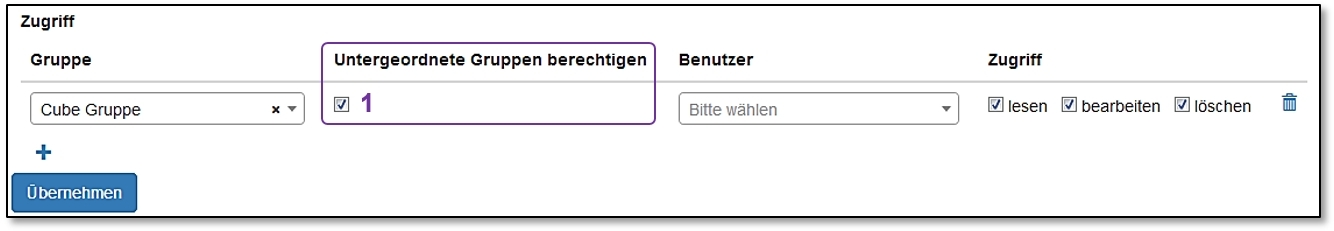
\includegraphics[width=1\linewidth]{../chapters/14_Benutzerverwaltung/pictures/14-3_Gruppenberechtigung.jpg}}
\caption{Bearbeitungsmodus der Gruppen}
% \label{fig:speciation}
\end{figure}
